
\section{Numerical implementation}

To solve the optimal control problem we will consider one gradient-based optimisation method. We implement the projected gradient methods, which has an infamous slow convergence rate. The implementation of Newton's method which is expected to have a superior convergence is described in Appendix \ref{Appendix}.

Both methods are gradient-based, and we need to consider the reduced optimal control problem. Let $S$ be the solution operator for our state system:  $S(u):=\theta(\placeholder ,T)$ i.e. it assigns the control to the final time solution of the state system. Then we can write our cost functional on reduced form, and our objective is then to minimize this reduced cost functional.
\begin{equation}
\label{eq:optimization_prob}
    \min_{u \in U}F(u) := J(S(u),u) = \frac{1}{2}\int_{\Omega}(S(u) - \theta_d)^2 \dx+ \frac{\gamma}{2}\int_0^Tu(t)^2\dt
\end{equation}

\iffalse
The operator S is compact. For every $u \in L^2(\Sigma)$ the state system admits a unique solution $\theta \text{ in } L^2(0,T;H^1(\Omega)) \cap C(0,T;L^2(\Omega)$, where $\theta_t \in L^2(0,T;H^1(\Omega)^{*})$. Due to the bound in Corollary 3.1.1 we have that for every $\delta \in (0,\frac{1}{2})$, there exist a constant $k_{\delta}$ such that 
\begin{equation*}
    ||S(u)||_{H^{\delta}(\Omega)} \leq k_{\delta}||u||_{L^2(\Sigma)} \text{ } \forall u \in L^2(\Sigma).
\end{equation*}
As $H^{\delta}$ embeds compactly into $L^2(\Omega)$, $S$ is indeed compact \cite{primal_dual}. 
\fi


\subsection{Solution of the State- and Adjoint equations}

The state equation and the adjoint equations were both solved numerically with the finite element method, using the finite element programming framework \verb|FEniCS| \cite{fenics} in Python.


\subsubsection{State equation}

For solving the state equation system \eqref{eq:heat} we discretise $\theta$ in time using explicit Euler:
\begin{equation*}
    \theta_t \approx \frac{\theta^{n+1} - \theta^n}{\Delta t}.
\end{equation*}
This is inserted into the equation \eqref{eq:heat-in-omega}. As $\theta^{n+1}$ is the unknown we denote it simply by $\theta$. This gives
\begin{equation*}
    \theta - \bar{\alpha}\Delta \theta = \theta^n, \quad\textrm{where}\quad \bar{\alpha} = \alpha\Delta t,
\end{equation*}
where $\alpha$ is the thermal diffusivity defined in the previous section. We now multiply with a test function $v\in H^1(\Omega)$, and integrate over the domain to get
\begin{equation*}
    \int_\Omega \theta v \dx - \bar{\alpha}\int_\Omega \Delta\theta\dx = \int_\Omega \theta^n v\dx.
\end{equation*}
For the implementation it is convenient to combine the two Neumann boundary conditions \eqref{eq:state-system-bd-1} and \eqref{eq:state-system-bd-2} into the following expression:
\begin{equation*}
    -k\frac{\partial \theta}{\partial n} = \beta(x)u(t)(\theta - \theta_w) \quad\text{where}\quad \beta(x) = \chi_{\Gamma_1},
\end{equation*}
where we have used an indicator function in the definition of $\beta$.
Partial integration then lead to the weak form
\begin{equation*}
\begin{aligned}
    \int_\Omega \theta v\dx + \bar{\alpha}\int_\Omega\nabla\theta\nabla v\dx &+ \frac{\bar{\alpha}}{k}\int_{\partial\Omega}\beta(x)u(t)\theta v\ds \\
    &= \int_\Omega\theta^n v\dx + \frac{\bar{\alpha}}{k}\int_{\partial\Omega}\beta(x)u(t)\theta_w v\ds.
\end{aligned}
\end{equation*}
The left hand side is a bilinear map and the right hand side is a linear functional, so we write
\begin{equation*}
    a_S(\theta, v) = L_S(v; \theta^n).
\end{equation*}
In the implementation we set $\theta^0$ using the initial condition given in the system \eqref{eq:heat}, and solve the equation above iteratively forward in time.

\subsubsection{Adjoint equation}

The adjoint system \eqref{eq:adjoint-system} is solved backwards in time. For the time discretization of $p$ we again use explicit Euler, so we let 
\begin{equation*}
 p_t \approx \frac{p^{n+1} - p^n}{\Delta t}.
\end{equation*}
Since the equation is solved backwards in time it is now $p^n$ that is the unknown, so we denote this by $p$ and insert it into the adjoint system \eqref{eq:adjoint-system-eqn}. We then get
\begin{equation*}
    p - \bar{\alpha}\Delta p =  p^{n+1}.
\end{equation*}
% Now multiply with a test function $v\in H^1(\Omega)$ and integrate over the spatial domain to get
% \begin{equation*}
% \int_\Omega pv\dx - \Delta t\frac{k}{\rho c_p}\int_\Omega % \Delta p v \dx = \int_\Omega p^{n+1} v \dx
% \end{equation*}
Again we combine the two Neumann boundary conditions \eqref{eq:adjoint-system-bd-1} and \eqref{eq:adjoint-system-bd-2} into one expression:
\begin{equation*}
    -k\frac{\partial p}{\partial n} = \beta(x)u(t)p,
\end{equation*}
with $\beta$ as defined above. Once more, we multiply with a test function $v\in H^1(\Omega)$ and integrate over the spatial domain. The partial integration then leads to the weak form
\begin{equation*}
    \int_\Omega pv\dx + \bar{\alpha} \int_\Omega \nabla p \nabla v \dx + \frac{\bar{\alpha}}{k}\int_{\partial\Omega} \beta(x)u(t)pv \ds  = \int_\Omega p^{n+1}v\dx.
\end{equation*}
For the \verb|FEniCS| implementation we let the left hand side and the right hand side be the bilinear and linear form respectively, and we write
\begin{equation*}
    a_A(p, v) = L_A(v; p^{n+1}).
\end{equation*}
For the implementation we initialize $p^{T/\Delta t}$ using the end time conditions in the adjoint system \eqref{eq:adjoint-system}, and then solve the system above at each time step, backwards in time.


\subsection{Projected Gradient Descent}\label{proj_grad}

The idea of a descent method is to iteratively approach an optimal control. This is done through starting with some initial guess $u_0$, and then finding some \emph{descent direction} $d_k$ and an associated step size $a_k$ at a given iteration $k$, where our control will then be given by $u_{k+1} = u_{k} + a_k d_k$. One obvious requirement is thus
\begin{equation*}
    F(u_k + \alpha_kd_k) < F(u_k).
\end{equation*}
Using the Taylor expansion of $F$ around $u_k$, we get a way to choose the descent direction:
%typically one can take different means to decide this, but a descent direction can in general be chosen by 
\begin{equation*}
    d_k = \arg\min_{\|d\|_U=1} \langle \nabla F(u_k), d \rangle_U.
\end{equation*}
Gradient descent gets its name from choosing the descent direction by setting $d_k = -\nabla F(u_k)$.

Next, one need to determine how far to go in that direction. This is denoted by $\alpha_k$, called the step length, or the \textit{line search} parameter. The ideal such parameter is 
\begin{equation*}
    a_k = \arg \min_{\alpha>0} \{ F(u_k + \alpha d_k) \}.
\end{equation*}
There are different ways to choose this line search step. One require a couple of properties to be satisfied these are
\begin{align*}
    F(u_k + \alpha_kd_k) < F(u_k) \text{  } \quad\forall k \\
    F(uk + \alpha_k d_k) - F(u_k) \rightarrow 0 \text{ as } k\rightarrow \infty.
\end{align*}
We stick with Armijo rule as our line search strategy. This method consists of given a descent direction $d_k$ of F at $u_k$, choose the largest $a_k \in \{ \beta^0, \beta, \beta^2,..,\beta^m,... \}$ such that
\begin{equation}\label{eq:armijo}
    F (u_k + \alpha_kd_k) - F(u_k) \leq \mu \alpha_k \langle \nabla F(u_k),d_k \rangle_{U}
\end{equation}
where $\mu,\beta  \in (0,1)$ are chosen constant, that is we use backtracking to determine the stepsize \cite{iterativeMethods}. We set $\mu = 10^{-4}$ and $\beta = \frac{1}{2}$. More facts about Armijo rule and the convergence properties of this line search strategy is in \cite{numMethods, iterativeMethods}.

We need to ensure the computed control is within the admissible set of controls $U_{\textrm{ad}}$. In our case, we have box constraints given in \eqref{eq:box_constraints}, that is we have a lower bound $u_a$ and upper bound $u_b$ for the control variable. We use a projection onto the set of admissible controls, explaining the name \emph{projected gradient descent method}. We use a simple cut-off function, i.e. a projection given by
\begin{equation}
    \label{eq:projection}
    \mathbb{P}_{[u_a,u_b]}(v) := \max \{u_a, \min \{u_b,v \} \}
\end{equation}
If $u_a$ and $u_b$ are vectors, the equality should be read component-wise. Notation is similar to that found in \cite{Algorithms}. The projection must be implemented in every step of the gradient descent method and Armijo's rule. That is we consider the projected Armijo's rule given by 

\begin{align*}
    \text{Determine $\alpha_k \in \{1, \frac{1}{2},\frac{1}{4},.. \}$ such that }\\
    F \bigg (\mathbb{P}_{[u_a,u_b]}(u_k + \alpha_kd_k) \bigg ) - F(u_k) \leq \mu \alpha_k \langle \nabla F(u_k),d_k \rangle_{U}
\end{align*}


A pseudocode for the whole Projected Gradient Descent method is shown in Algorithm 1. We introduce two stopping criterions: one based on the minimum allowed step length, and one on the difference in the computed values of the control given by 
\begin{equation}
    \label{eq:stopping}
    \tau := \|u^{(k+1)} - u^{(k)}\|_U 
\end{equation}
This is to check that the controls converge towards a value, $U$ being the space of the controls. When $\tau$ becomes smaller than some predetermined value, abort the procedure and return the result.


\begin{codebox}
\Procname{$\proc{Algorithm 1: Projected Steepest Descent with Armijo}$}
\li Choose initial value $u^{(0)}\in U_{ad}$
\li Set tolerance $\id{tol}$ and $\alpha_{min}$
\li Solve state system to obtain $\theta^{(0)}$, with $u^{(0)}$
\li Solve adjoint system to obtain $p^{(0)}$, with $u^{(0)}$ and $p^{(0)}$
\li $k=0$
\li \While ($\tau > \id{tol}$)  \Then
\li Choose the descent Direction $d_k = -\nabla F(u^{(k)})$
\li Use the Projected Armijo rule to determine $\alpha_k$
\li \If $\alpha_k < \alpha_{min}$ \Then 
\li \textbf{Break} \End
\li Set $u^{(k+1)} = \mathbb{P}_{[u_a,u_b]}\bigg (u^{(k)} + \alpha_k d_k \bigg )$
\li Solve state system to obtain $\theta^{(k+1)}$, with $u^{(k+1)}$
\li Solve adjoint system to obtain $p^{(k+1)}$, with $u^{(k+1)}$ and $\theta^{(k+1)}$
\li Compute $\tau$
\li $k = k +1$
\end{codebox}

The gradient of our reduced cost functional is given by
%
\begin{equation*}
    \nabla F(u) =  \gamma u - \frac{1}{\rho c_p} \int_{\Gamma_1} (\theta - \theta_w)p \ds = 0
\end{equation*}
%

%Er ikke helt sikker på det under, så vi kan sikkert bare droppe det 
%The projected gradient descent method is globally convergent if the reduced cost functional $F$ is Fréchet differentiable and bounded from below.As the solution to the state system $S(u) \in W(0,T) \cap C(\bar{Q})$, $F$ is indeed Fréchet differentiable. Moreover, we have that $F(u) \geq 0$ for all choices of controls $u \in U_{ad}$ by the definition of $F(u)$. Therefore, we have global convergence. However, 
This is a first-order descent method, and the convergence rate is typically very slow, as it solely relies on first-order gradient information. We expect to see big improvements when the control $u_k$ is far from the optimal, with diminishing improvements as we get closer and closer to $\bar{u}$. This behaviour is confirmed by the results shown in figure \ref{fig:armijo}. Here, we first solved the state equation with $u(t) = 1/2$, and used the mean temperature at $t=T$ from this solution as $\theta_d$. We then ran Algorithm 1 (implemented in Python) with initial guess $u^{(0)} = 0.1$, regularisation parameter $\gamma = 1$, minimum allowable normed difference between iterations $\id{tol} = 10^{-10}$, and minimum allowable step length $\alpha_{\min} = 2^{-40}$.\footnote{The values for $\id{tol}$ and $\alpha_{\min}$ are perhaps too small, and could be increased to speed up the algorithm.} The Armijo parameter from \eqref{eq:armijo} was set to $\mu=10^{-4}$. This algorithm reached a value for the control of $0.4903$ after 2 steps, an absolute relative difference of less than 2\% with respect to the correct value of $0.5$. After 9 steps the step length became unacceptably short, and the algorithm terminated with a final value of $u=0.5038$, about 0.8\% away from the correct answer. A complete summary of the values computed by the algorithm are shown in table \ref{table:armijo}. 
\begin{figure}[pb]
    \centering
    \begin{subfigure}[b]{\textwidth}
        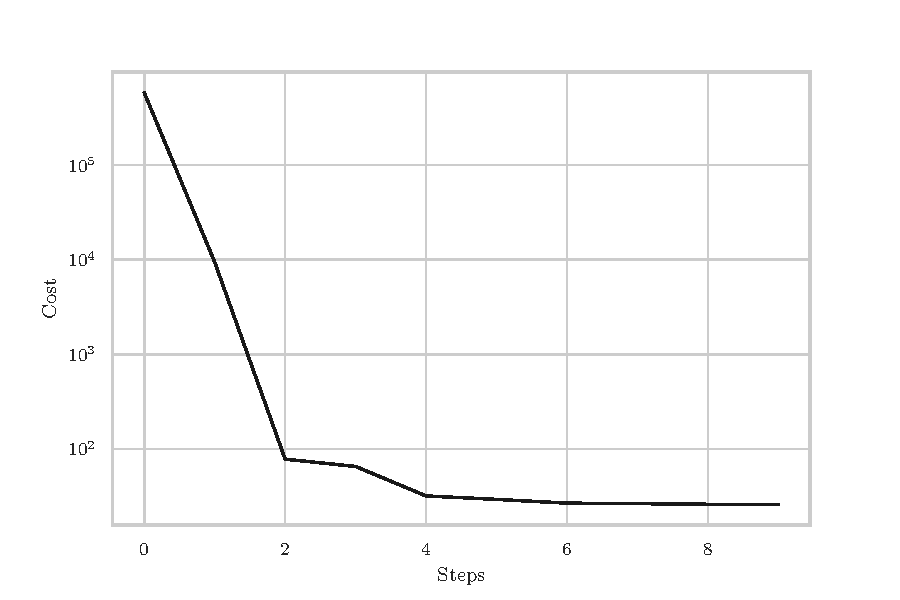
\includegraphics[width=\textwidth]{figures/cost_armijo_analytic_05.pdf}
        \caption{}
        \label{fig:armijo_cost}
    \end{subfigure}
    \begin{subfigure}[b]{\textwidth}
        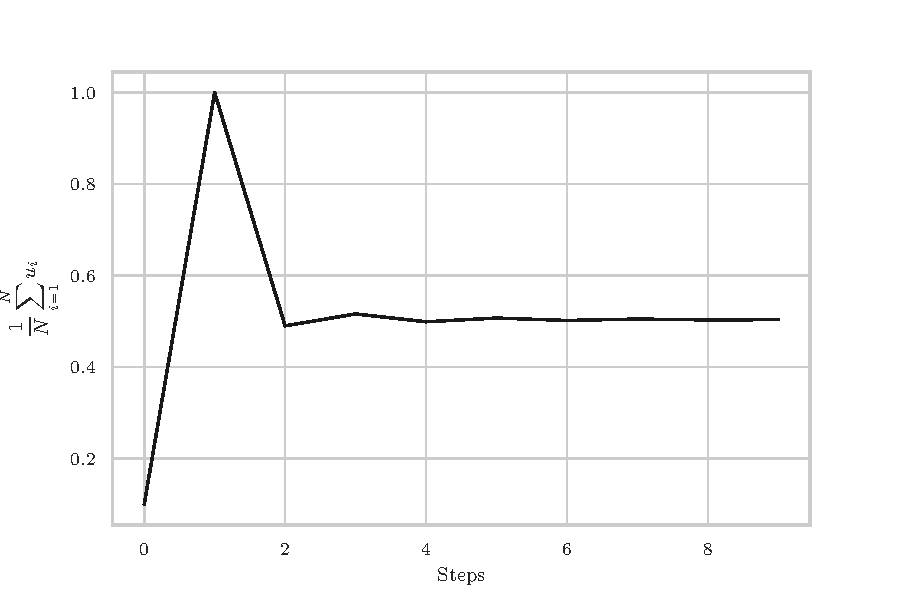
\includegraphics[width=\textwidth]{figures/U_armijo_analytic_05.pdf}
        \caption{}
        \label{fig:armijo_control}
    \end{subfigure}
    \caption{Plots showing (a) the value of the cost-function on a $\log$-scale, and (b) the associated control determined by each step of the Gradient descent algorithm with the Armijo rule. The control used to generate the desired temperature was $u(t) = 1/2$.}
    \label{fig:armijo}
\end{figure}
\begin{table}
    \centering
    \caption{Values computed by Gradient descent with the Armijo rule.}
    \label{table:armijo}
    \begin{tabular}{@{}lrSS}
         \toprule
    Step ($k$) & Step length ($\alpha$) & \multicolumn{1}{c}{Control ($u^{(k)}$)} & \multicolumn{1}{c}{$\tau = \|u^{(k-1)} - u^{(k)} \|_{\mathcal{U}}$} \\ \midrule
    0 &  & 0.1 &  \\
    1 & $2^{-13}$ & 1.0 & 6.42729 \\
    2 & $2^{-5}$ & 0.49035 & 3.63966 \\
    3 & $2^{-12}$ & 0.5162 & 0.18464 \\
    4 & $2^{-12}$ & 0.49911 & 0.12203 \\
    5 & $2^{-12}$ & 0.5073 & 0.0585 \\
    6 & $2^{-12}$ & 0.50203 & 0.03768 \\
    7 & $2^{-12}$ & 0.50511 & 0.02205 \\
    8 & $2^{-12}$ & 0.50318 & 0.01384 \\
    9 & $2^{-13}$ & 0.50376 & 0.00419 \\ \bottomrule
    \end{tabular}
\end{table}